\documentclass[noinstructornotes]{ximera}
%handout:  for handout version with no solutions or instructor notes
%handout,instructornotes:  for instructor version with just problems and notes, no solutions
%noinstructornotes:  shows only problem and solutions

%% handout
%% space
%% newpage
%% numbers
%% nooutcomes

%I added the commands here so that I would't have to keep looking them up
%\newcommand{\RR}{\mathbb R}
%\renewcommand{\d}{\,d}
%\newcommand{\dd}[2][]{\frac{d #1}{d #2}}
%\renewcommand{\l}{\ell}
%\newcommand{\ddx}{\frac{d}{dx}}
%\everymath{\displaystyle}
%\newcommand{\dfn}{\textbf}
%\newcommand{\eval}[1]{\bigg[ #1 \bigg]}

%\begin{image}
%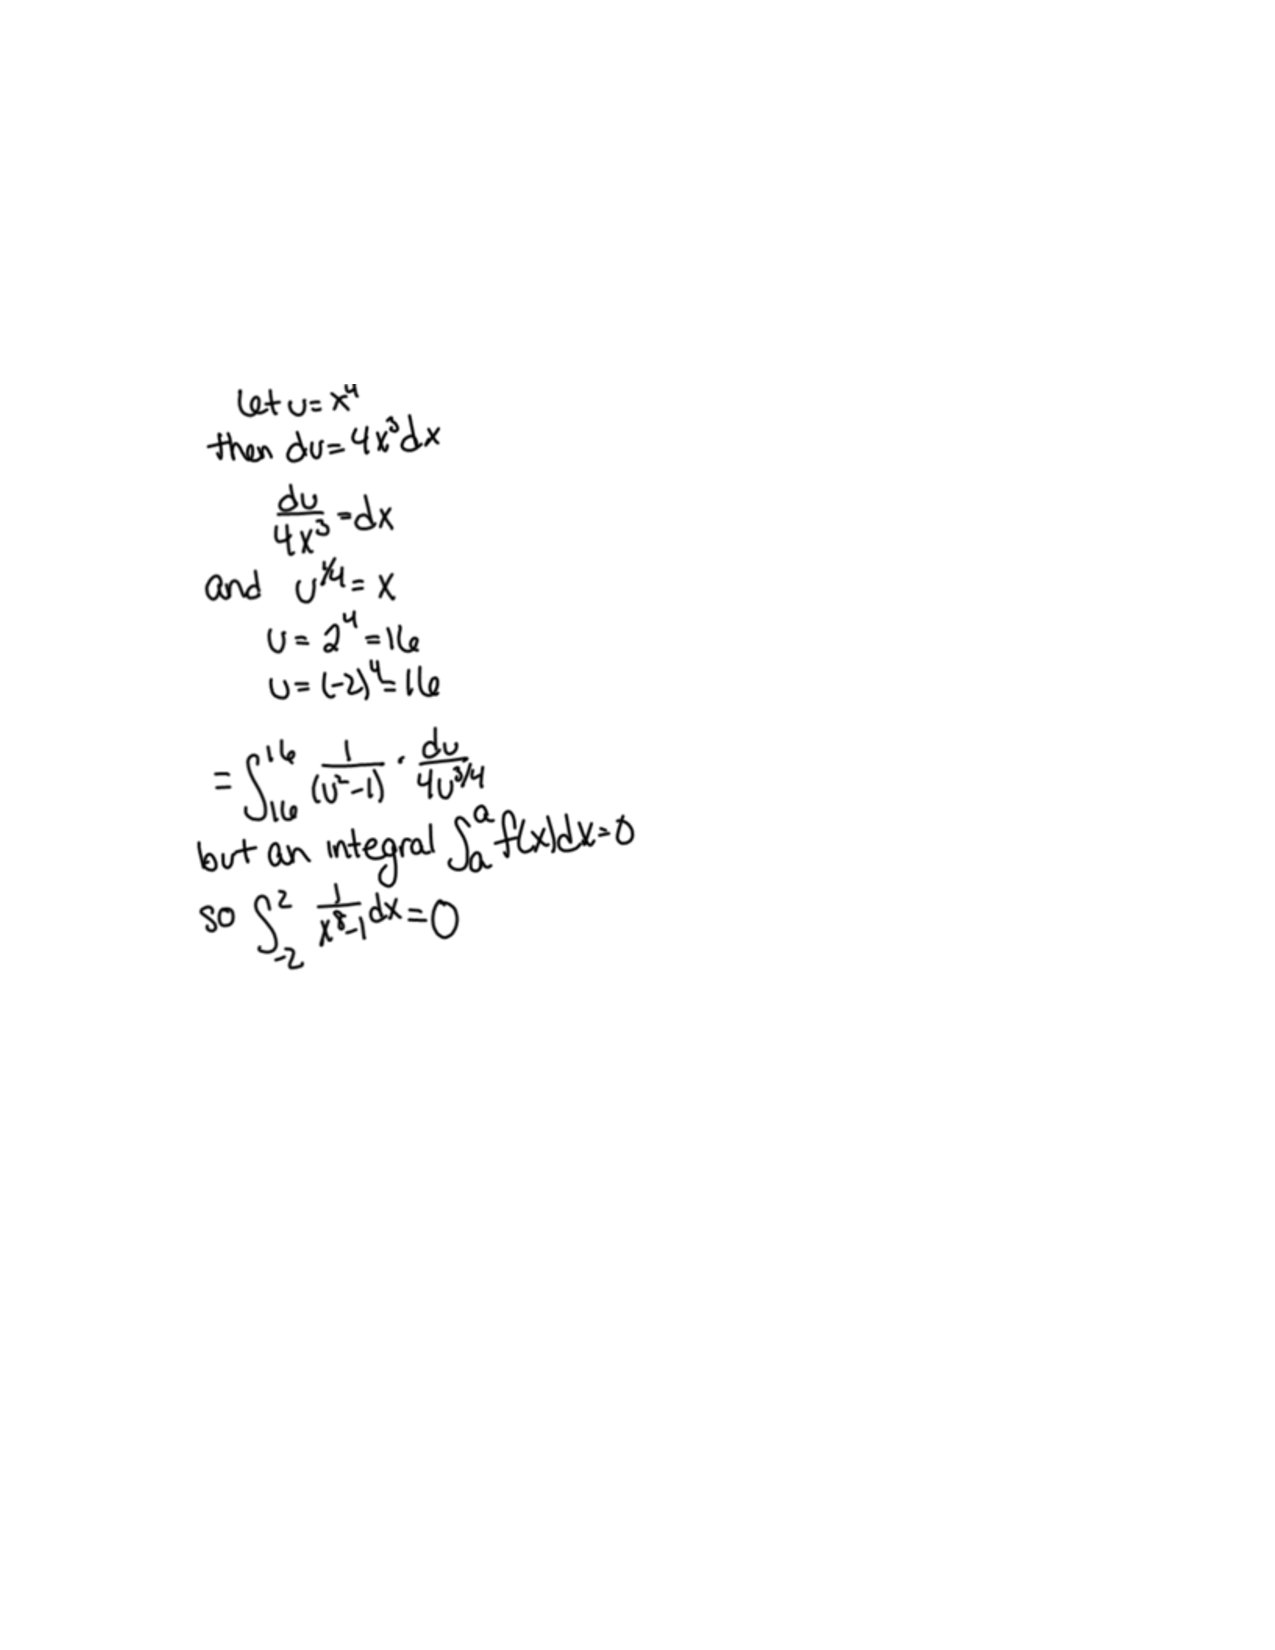
\includegraphics[trim= 170 420 250 180]{Figure1.pdf}
%\end{image}

%add a ``.'' below when used in a specific directory.
\newcommand{\RR}{\mathbb R}
\renewcommand{\d}{\,d}
\newcommand{\dd}[2][]{\frac{d #1}{d #2}}
\renewcommand{\l}{\ell}
\newcommand{\ddx}{\frac{d}{dx}}
\newcommand{\dfn}{\textbf}
\newcommand{\eval}[1]{\bigg[ #1 \bigg]}

\usepackage{multicol}

\renewenvironment{freeResponse}{
\ifhandout\setbox0\vbox\bgroup\else
\begin{trivlist}\item[\hskip \labelsep\bfseries Solution:\hspace{2ex}]
\fi}
{\ifhandout\egroup\else
\end{trivlist}
\fi} %% we can turn off input when making a master document

\title{Recitation \#20: Properties of power series - Solutions}  

\begin{document}
\begin{abstract}		\end{abstract}
\maketitle



\section{Warm up:}
Suppose that $\sum_{k=0}^\infty c_k (x+5)^k$ converges when $x=-9$ and diverges when $x=-1$.  
What can be said about the convergence and divergence of the following series?
	\begin{multicols}{3}
	\begin{enumerate}
	\item  $\sum_{k=0}^\infty c_k$
	\item  $\sum_{k=0}^\infty c_k (-5)^k$
	\item  $\sum_{k=0}^\infty c_k (5)^k$
	\end{enumerate}
	\end{multicols}
	
	\begin{freeResponse}
	 What is important to note first is that the interval of convergence for the series $\sum_{k=0}^\infty c_k (x+5)^k$ is $[-9,-1)$. 
	
	\begin{enumerate}
	\item  Notice that
		\[
		\sum_{k=0}^\infty c_k = \sum_{k=0}^\infty c_k (-4+5)^k.
		\]
	Then since $-4$ is in the interval $[-9,-1)$, the series $\sum_{k=0}^\infty c_k$ converges.
	
	\item  Since $-10$ is not in the interval $[-9,-1)$, the series
		\[
		 \sum_{k=0}^\infty c_k (-5)^k = \sum_{k=0}^\infty c_k (-10+5)^k
		\]
	diverges.
	
	\item  Since $0$ is not in the interval $[-9,-1)$, the series
		\[
		\sum_{k=0}^\infty c_k 5^k = \sum_{k=0}^\infty c_k (0+5)^k
		\]
	diverges.
	\end{enumerate}
	\end{freeResponse}
	
\begin{instructorNotes}
Students need to recognize that the interval of convergence (IOC) emanates equally out from the center (where $(x-a)^k = 0$), going the same distance in each direction, with the endpoints possibly varying.
\end{instructorNotes}







\section{Group work:}



%problem 1
\begin{problem}
If the series $\sum_{k=0}^\infty a_k (x-2)^k$ has an interval of convergence of $[-4,8)$, determine the interval of convergence of the following series:
	\begin{multicols}{3}
	\begin{enumerate}
	\item  $\sum_{k=300}^\infty a_k (x-2)^k$
	\item  $\sum_{k=0}^\infty a_k x^k$
	\item  $\sum_{k=0}^\infty \left( a_k (x-2)^k + \left( \frac{1}{7} \right)^k x^k \right)$
	\end{enumerate}
	\end{multicols}
	
	\begin{freeResponse}
	\begin{enumerate}
	\item  This series has exactly the same interval of convergence, $\boxed{[-4,8)}$, since a finite number of terms do not change whether or not a series converges.
	
	\item  In the original interval of convergence $[-4,8)$, the center is $x=2$ and the radius of convergence is $6$ (which includes the left endpoint, but not the right).  
	So now, the center is $x=0$.  
	Taking an interval about $0$ with radius $6$, and adding in the left endpoint, gives the IOC of $\boxed{[-6,6)}$.  
	
	\item  The interval of convergence of this series is the intersection of the interval of convergence for $\sum_{k=0}^\infty a_k (x-2)^k$ and $\sum_{k=0}^\infty \left( \frac{1}{7} \right)^k x^k$.  
	To find the IOC for this second series, we use the Root Test.
		\begin{align*}
		\lim_{k \to \infty} \sqrt[k]{\biggr| \left( \frac{1}{7} \right)^k x^k \biggr| }  
		&= \lim_{k \to \infty} \frac{1}{7} |x|  \\
		&= \frac{1}{7} |x|.
		\end{align*}
	So the series $\sum_{k=0}^\infty \left( \frac{1}{7} \right)^k x^k$ converges when 
		\begin{align*}
		&\frac{1}{7} |x| < 1  \\
		\Longrightarrow 	\qquad	&|x| < 7  \\
		\Longrightarrow 	\qquad	&-7 < x < 7.
		\end{align*}
	We need to test the endpoints $x = \pm 7$, but using the divergence test we see that both
		\[
		\sum_{k=0}^\infty (-1)^k 	\qquad	\text{and}	\qquad	\sum_{k=0}^\infty 1^k
		\]
	diverge.  
	Therefore, the interval of convergence for $\sum_{k=0}^\infty \left( \frac{1}{7} \right)^k x^k$ is $(-7,7)$.
	
	Finally, the interval of convergence for the series
		\[
		\sum_{k=0}^\infty \left( a_k (x-2)^k + \left( \frac{1}{7} \right)^k x^k \right)
		\]
	is
		\[
		[-4,8) \cap (-7,7) = \boxed{[-4,7)}.
		\]
	\end{enumerate}
	\end{freeResponse}
	
\end{problem}

\begin{instructorNotes}
Part (a) should be quick as it is just the idea that only the ``tail'' matters, part (b) is to show the students what it does to shift the center, and part (c) is to have them intersect the intervals of convergence for two power series.
\end{instructorNotes}







%problem 2
\begin{problem}
For each of the following, find the domain of $f(x)$ (i.e. find the interval of convergence).
	\begin{multicols}{2}
	\begin{enumerate}
	\item  $f(x) = \sum_{k=1}^\infty \frac{(3x-2)^k}{k \cdot 3^k}$
	\item  $f(x) = \sum_{k=0}^\infty \frac{(-1)^k}{\sqrt{k^2+1}} x^k$
	\item  $f(x) = \sum_{k=2}^\infty \frac{x^{3k+2}}{(\ln k)^k}$
	\end{enumerate}
	\end{multicols}
	
	\begin{freeResponse}
	\begin{enumerate}
	\item  We use the Ratio Test
		\begin{align*}
		\lim_{k \to \infty} \biggr| \frac{(3x-2)^{k+1}}{(k+1) 3^{k+1}} \cdot \frac{k \cdot 3^k}{(3x-2)^k} \biggr|
		&= \lim_{k \to \infty} \biggr| \frac{k (3x-2)}{3(k+1)} \biggr|  \\
		&= \biggr| \frac{3x-2}{3} \biggr| = \frac{|3x-2|}{3}.
		\end{align*}
	We know that this series converges when
		\begin{align*}
		&\frac{|3x-2|}{3} < 1  \\
		\Longrightarrow 	\qquad	&|3x-2|<3  \\
		\Longrightarrow 	\qquad	&-3 < 3x-2 < 3  \\
		\Longrightarrow 	\qquad	&-1 < 3x < 5  \\
		\Longrightarrow 	\qquad	&- \frac{1}{3} < x < \frac{5}{3}.
		\end{align*}
	
	We still need to check the endpoints.  
	When $x = - \frac{1}{3}$ we have
		\begin{align*}
		\sum_{k=1}^\infty \frac{1}{k3^k} \left( 3 \left( - \frac{1}{3} \right) - 2 \right)^k  
		&= \sum_{k=1}^\infty \frac{(-3)^k}{k 3^k}  \\
		&= \sum_{k=1}^\infty \frac{(-1)^k}{k}
		\end{align*}
	which converges (conditionally) by the alternating series test.  
	
	When $x = \frac{5}{3}$ we have
		\begin{align*}
		\sum_{k=1}^\infty \frac{1}{k3^k} \left( 3 \left( \frac{5}{3} \right) - 2 \right)^k  
		&= \sum_{k=1}^\infty \frac{3^k}{k 3^k}  \\
		&= \sum_{k=1}^\infty \frac{1}{k}
		\end{align*}
	which diverges since it is the Harmonic series.
	
	Therefore, the interval of convergence is $\boxed{\left[ - \frac{1}{3}, \frac{5}{3} \right)}$.  
	
	
	
	\item  We again apply the Ratio Test
		\begin{align*}
		\lim_{k \to \infty} \biggr| \frac{(-1)^{k+1} x^{k+1}}{\sqrt{(k+1)^2 + 1}} \cdot \frac{\sqrt{k^2 + 1}}{(-1)^k x^k} \biggr|  
		&= \lim_{k \to \infty} \biggr| \frac{ x \sqrt{k^2 + 1}}{\sqrt{k^2 + 2k + 2}} \biggr|  \\
		&= |x|.
		\end{align*}
	So we know that this series converges when
		\[
		|x| < 1 \qquad \Longleftrightarrow \qquad -1 < x < 1.
		\]
		
	We still need to check the endpoints.  
	When $x = -1$, the series
		\[
		\sum_{k=0}^\infty \frac{1}{\sqrt{k^2+1}}
		\]
	diverges by the Limit Comparison Test (compare with $\sum_{k=1}^\infty \frac{1}{k}$).  
	
	When $x=1$, the series
		\[
		\sum_{k=0}^\infty \frac{(-1)^k}{\sqrt{k^2+1}}
		\]
	converges conditionally by the alternating series test.  
	
	Therefore, the interval of convergence is $\boxed{(-1,1]}$.  
	
	
	
	\item  For this series we apply the Root Test
		\begin{align*}
		\lim_{k \to \infty} \sqrt[k]{\biggr| \frac{x^{3k+2}}{(\ln k)^k} \biggr| }
		&= \lim_{k \to \infty} \frac{|x|^3 \cdot |x|^{\frac{2}{k}}}{\ln k}  \\
		&= |x|^3 \cdot \lim_{k \to \infty} \frac{|x|^{\frac{2}{k}}}{\ln k}  \\
		&= |x|^3 \cdot 0 = 0.
		\end{align*}
	Therefore, the interval of convergence is $\boxed{ ( -\infty, \infty)}$.  
	\end{enumerate}
	\end{freeResponse}
		
\end{problem}

\begin{instructorNotes}
These are fairly standard ``determine the IOC'' problems (using ratio and/or root test).  
Be sure that the endpoints are checked.  
Skip one of these if short on time.
\end{instructorNotes}







%problem 3
\begin{problem}
In each of the following, give a power series (with an interval of convergence) for the given function.  
Assume that we know $\sum_{k=0}^\infty x^k = \frac{1}{1-x}$ on $(-1,1)$.  
	\begin{multicols}{2}
	\begin{enumerate}
	\item  $f(x) = \frac{3}{5x-2}$
	\item  $f(x) = \frac{3x^4}{5x^3 - 2}$
	\end{enumerate}
	\end{multicols}
	
	\begin{freeResponse}
	\begin{enumerate}
	\item  
		\begin{align*}
		f(x) &= \frac{3}{5x-2}  \\
		&= \frac{3}{-2 \left( 1 - \left( \frac{5}{2} x \right) \right) }  \\
		&= - \frac{3}{2} \sum_{k=0}^\infty \left( \frac{5}{2} x \right)^k  \\
		&= \boxed{\sum_{k = 0}^\infty \left( - \frac{3}{2} \right) \left( \frac{5}{2} x \right)^k}.
		\end{align*}
	Since this is a geometric series, it converges if and only if
		\begin{align*}
		&\biggr| \frac{5}{2} x \biggr| < 1  \\
		\Longleftrightarrow  \qquad  &|x| < \frac{2}{5}  \\
		\Longleftrightarrow  \qquad  &- \frac{2}{5} < x < \frac{2}{5}.
		\end{align*}
	Therefore, the interval of convergence is $\boxed{ \left( - \frac{2}{5}, \frac{2}{5} \right) }$
	
	\item  
		\begin{align*}
		f(x) &= \frac{3x^4}{5x^3-2}  \\
		&= \frac{- 3x^4}{2} \cdot \frac{1}{1 - \left( \frac{5}{2} x^3 \right) }  \\
		&= - \frac{3}{2} x^4 \sum_{k=0}^\infty \left( \frac{5}{2} x^3 \right)^k  \\
		&= \boxed{ \sum_{k=0}^\infty \left( - \frac{3}{2} \right) \left( \frac{5}{2} \right)^k x^{3x+4}}.
		\end{align*}
	This geometric series converges if and only if
		\begin{align*}
		&\biggr| \frac{5}{2} x^3 \biggr| < 1  \\
		\Longleftrightarrow  \qquad  &|x^3| < \frac{2}{5}  \\
		\Longleftrightarrow  \qquad  &|x| < \sqrt[3]{\frac{2}{5}}  \\
		\Longleftrightarrow  \qquad  &- \sqrt[3]{\frac{2}{5}} < x < \sqrt[3]{\frac{2}{5}}.
		\end{align*}
	Therefore, the interval of convergence is $\boxed{\left( - \sqrt[3]{\frac{2}{5}}, \sqrt[3]{\frac{2}{5}} \right)}$.
	
	\end{enumerate}
	\end{freeResponse}

\end{problem}

\begin{instructorNotes}
The series here evolve in order, with one change made each time.  
You may want to do as a whole class discussion.  
The key is to rewrite the function in the form $\frac{1}{1-g(x)}$ with the emphasis on the ``1'' and the ``-'' in the denominator.
\end{instructorNotes}







%problem 4
\begin{problem}
Consider $f(x) = \sum_{k=0}^\infty \frac{2^k x^k}{(k+1)^3}$.
	\begin{enumerate}
	\item  Write out $p_3(x)$, the cubic polynomial which is the first three terms of this power series.
	
	\item  Find $p_3'(x)$ and $f'(x)$ and compare your answers.
	
	\item  Find $\int p_3(x) \d x$ and $\int f(x) \d x$ and compare your answers.
	\end{enumerate}
	
	\begin{freeResponse}
	\begin{enumerate}
	\item
		\begin{align*}
		p_3(x) &= 
		\frac{2^0 x^0}{(0+1)^3} + \frac{2^1 x^1}{(1+1)^3} + \frac{2^2 x^2}{(2+1)^3} + \frac{2^3 x^3}{(3+1)^3}  \\
		&= \boxed{1 + \frac{2x}{2^3} + \frac{4x^2}{3^3} + \frac{8x^3}{4^3}}.
		\end{align*}
		
		
	
	\item  
		\[
		p_3'(x) = \boxed{0 + \frac{2}{2^3} + \frac{2 \cdot 4}{3^3}x + \frac{3 \cdot 8}{4^3}x^2}.
		\]
		
		\begin{align*}
		f'(x) &= 
		\sum_{k=0}^\infty \frac{2^k}{(k+1)^3} \cdot k \cdot x^{k-1}  \\
		&= \sum_{k=1}^\infty \frac{k \cdot 2^k}{(k+1)^3} x^{k-1} 	\quad	{\color{red}\text{Since the k=0 term is 0.}}  \\
		&= \boxed{\sum_{\ell=0}^\infty \frac{(\ell + 1)2^{\ell + 1}}{(\ell + 2)^3} x^\ell }	\quad	{\color{red}\text{reindexing with }\ell = k-1}
		\end{align*}
	Note that this sum agrees with $p_3'(x)$ when $\ell = 0$, $1$, and $2$.
	
	
	
	\item  
		\[
		\int p_3(x) \d x = \boxed{x + \frac{2x^2}{2^4} + \frac{4x^3}{3^4} + \frac{8x^4}{4^4} + C}.
		\]
		
		\begin{align*}
		\int f(x) \d x
		&= \int \sum_{k=0}^\infty \frac{2^k x^k}{(k+1)^3} \d x  \\
		&= \sum_{k=0}^\infty \frac{2^k}{(k+1)^3} \cdot \left( \int x^k \d x \right)  \\
		&= \sum_{k=0}^\infty \left( \frac{2^k}{(k+1)^3} \cdot \frac{1}{k+1} \cdot x^{k+1} \right) + C  \\
		&= \sum_{\ell = 1}^\infty \left( \frac{2^{\ell - 1}}{\ell^4} x^\ell \right) + C 	\quad	{\color{red}\text{reindexing with }\ell = k+1.}
		\end{align*}
	Note again that this sum agrees with $\int p_3 (x) \d x$ when $\ell = 0$, $1$, $2$, and $3$ (as it should).
	\end{enumerate}
	\end{freeResponse}

\end{problem}

\begin{instructorNotes}
Students often have a difficult time seeing that differentiating or integrating a power series comes down to knowing how to differentiate or integrate a polynomial term-by-term.  
Hopefully the ``term-by-term'' process will connect with them when differentiating and integrating $p_3(x)$.  
This will be extended in Sections 10.3 and 10.4 as well.
\end{instructorNotes}







%problem 5
\begin{problem}
Give a power series (with interval of convergence) for the given functions.
	\begin{multicols}{3}
	\begin{enumerate}
	\item  $f(x) = \frac{1}{1+x^2}$
	\item  $f(x) = \tan^{-1}(x)$
	\item  $f(x) = \tan^{-1}(3x^2)$
	\end{enumerate}
	\end{multicols}
	
	\begin{freeResponse}
	\begin{enumerate}
	\item
		\begin{align*}
		f(x) &= \frac{1}{1+x^2}  \\
		&= \sum_{k=0}^\infty (-x^2)^k  \\
		&= \boxed{\sum_{k=0}^\infty (-1)^k x^{2k}}
		\end{align*}
	when
		\begin{equation*}
		|-x^2| < 1 	\qquad	\Longleftrightarrow		\qquad	-1 < x < 1.
		\end{equation*}
	So the interval of convergence is $\boxed{(-1,1)}$.  
	
	
	
	\item  Notice that 
		\[
		f'(x) = \frac{1}{1+x^2} = \sum_{k=0}^\infty (-1)^k x^{2k}
		\]
	on the interval $(-1,1)$.  
	So
		\begin{align*}
		f(x) &= \int \left( \sum_{k=0}^\infty (-1)^k x^{2k} \right) \d x  \\
		&= \sum_{k=0}^\infty \left( \frac{(-1)^k}{2k+1} x^{2k+1} \right) + C.
		\end{align*}
	
	We know that this series converges (at least) on $(-1,1)$.
	We need to first find $C$, and then check the endpoints for convergence.
	
	To find $C$, just notice that
		\[
		0 = \arctan(0) = \sum_{k=0}^\infty \left( \frac{(-1)^k}{2k+1} 0^{2k+1} \right) + C = 0 + C.
		\]
	and so $C = 0$.  
	
	Now to check the endpoints, we plug in $-1$ and $1$.  
	When $x = -1$, we have the series
		\[
		\sum_{k=0}^\infty \frac{(-1)^{k+1}}{2k+1}	\qquad	{\color{red}x = -1}
		\]
`	and when $x=1$ the series is
		\[
		\sum_{k=0}^\infty \frac{(-1)^k}{2k+1}.	\qquad	{\color{red}x = 1}
		\]
	Both of these series converge conditionally by the Alternating Series Test.  
	Thus, 
		\[
		f(x) = \boxed{\sum_{k=0}^\infty \frac{(-1)^k}{2k+1} x^{2k+1}}
		\]
	with interval of convergence $\boxed{[-1,1]}$.  
	
	
	\item  By part (b), if $|3x^2| \leq 1$ then
		\[
		f(x) = \sum_{k=0}^\infty \frac{(-1)^k}{2k+1} (3x^2)^{2k+1} = \boxed{\sum_{k=0}^\infty \frac{(-1)^k 3^{2k+1}}{2k+1} x^{4k+2}}.
		\]
	This series converges when
		\begin{align*}
		&|3x^2| \leq 1  \\
		\Longrightarrow 	\qquad	&|x^2| \leq \frac{1}{3}  \\
		\Longrightarrow 	\qquad	&- \frac{1}{\sqrt{3}} \leq x \leq \frac{1}{\sqrt{3}}.
		\end{align*}
	So the interval of convergence is
		\[
		\boxed{ \left[ - \frac{1}{\sqrt{3}}, \frac{1}{\sqrt{3}} \right] }.
		\]
	
	\end{enumerate}
	\end{freeResponse}

\end{problem}

\begin{instructorNotes}
Just like above we use compositions of the geometric series, only this time we use differentiation or integration to write $f(x)$ as a geometric series.
\end{instructorNotes}
















	
	
	
	
	
	
	
	
	

	










								
				
				
	














\end{document} 


















